\documentclass[conference]{IEEEtran}
\IEEEoverridecommandlockouts
% The preceding line is only needed to identify funding in the first footnote. If that is unneeded, please comment it out.
\usepackage{float}
\usepackage{cite}
\usepackage{booktabs}
\usepackage{amsmath,amssymb,amsfonts}
\usepackage{algorithmic}
\usepackage{graphicx}
\usepackage{textcomp}
\usepackage{xcolor}
\usepackage{placeins}
\usepackage{enumitem}
\usepackage{array}
\usepackage{hyperref}
\usepackage{bookmark}
\usepackage[utf8]{inputenc}

\def\BibTeX{{\rm B\kern-.05em{\sc i\kern-.025em b}\kern-.08em
    T\kern-.1667em\lower.7ex\hbox{E}\kern-.125emX}}
\begin{document}

\title{The Impact of Demographics on Employment and Salary\\
{\footnotesize
  A Hypothesis Testing and Clustering Approach}
}

\author{\IEEEauthorblockN{Ciaran Otter}
\IEEEauthorblockA{\textit{Department of Computer science} \\
\textit{Principles of Data Science - CS771}\\
Stellenbosch University,
Stellenbosch, South Africa\\}
}
\maketitle
\section{Introduction and Project Goal}

This project investigates the relationship between demographic factors such as highest education level, age, gender, and ethnicity with employment status and salary in South Africa. 
Using real-world 2023 household survey data found through stats SA's interactive data portal: `Nesstar'~\cite{StatsSA_GHS2023}, his investigation aims to conduct statistical hypothesis testing to ascertain whether these factors significantly influence employment outcomes and salary levels in the contemporary South African context. 
Additionally, clustering techniques will be employed to uncover underlying patterns within the dataset.

The dataset comprises 112 variables, providing a comprehensive overview of household statistics within the South African population. However, for this analysis, we will focus on several key variables that are particularly relevant to our research objectives:
\begin{itemize}
    \item \textbf{Education level}
    \item \textbf{Employment status}
    \item \textbf{Salary}
    \item \textbf{Age}
    \item \textbf{Gender}
    \item \textbf{Ethnicity}
\end{itemize}

\subsection{Hypotheses}
To guide our investigation, we have formulated the following hypotheses regarding the influence of demographic factors on employment status and salary:


\subsection{Hypothesis 2: Education and Salary}
\textbf{Research Question:} Does an individual's level of education have a significant impact on their salary?

\begin{itemize}
    \item \textbf{Null Hypothesis ($H_0$):} Education level does not significantly influence salary.
    \item \textbf{Alternative Hypothesis ($H_1$):} Education level has a statistically significant effect on salary.
\end{itemize}


\subsection{Hypothesis 2: Education and Salary}
\textbf{Research Question:} Does an individual's level of education have a significant impact on their salary?

\begin{itemize}
    \item \textbf{Null Hypothesis ($H_0$):} Education level does not significantly influence salary.
    \item \textbf{Alternative Hypothesis ($H_1$):} Education level has a statistically significant effect on salary.
\end{itemize}


\subsection{Hypothesis 2: Education and Salary}
\textbf{Research Question:} Does an individual's level of education have a significant impact on their salary?

\begin{itemize}
    \item \textbf{Null Hypothesis ($H_0$):} Education level does not significantly influence salary.
    \item \textbf{Alternative Hypothesis ($H_1$):} Education level has a statistically significant effect on salary.
\end{itemize}


\subsection{Hypothesis 2: Education and Salary}
\textbf{Research Question:} Does an individual's level of education have a significant impact on their salary?

\begin{itemize}
    \item \textbf{Null Hypothesis ($H_0$):} Education level does not significantly influence salary.
    \item \textbf{Alternative Hypothesis ($H_1$):} Education level has a statistically significant effect on salary.
\end{itemize}


\subsection{Hypothesis 2: Education and Salary}
\textbf{Research Question:} Does an individual's level of education have a significant impact on their salary?

\begin{itemize}
    \item \textbf{Null Hypothesis ($H_0$):} Education level does not significantly influence salary.
    \item \textbf{Alternative Hypothesis ($H_1$):} Education level has a statistically significant effect on salary.
\end{itemize}


\section{Methodology and Implementation}

\subsection{Testing Methods}

A variety of statistical tests were employed to evaluate the impact of demographic factors on employment and salary outcomes. The methods applied are outlined below:

\paragraph{$\chi^2$ Test for Independence}
The $\chi^2$ test evaluates the association between two categorical variables. This test was applied to assess relationships between variables such as \textbf{education level}, \textbf{employment status}, \textbf{gender}, and \textbf{ethnicity}. It determines whether there is a significant dependence between these demographic factors and employment outcomes.

\paragraph{T-Test, ANOVA, and Welch’s Test}
For continuous variables like \textbf{salary} and \textbf{age}, t-tests and one-way ANOVA were used to compare means across categorical groups. ANOVA was utilized to identify statistically significant differences in means across three or more independent groups, particularly in analyzing relationships between factors like \textbf{education level} and \textbf{ethnicity}.

\paragraph{Q-Q Plot}
A Q-Q (Quantile-Quantile) plot is a graphical tool used to assess whether a dataset follows a particular theoretical distribution, typically the normal distribution. By plotting the quantiles of the sample data against the quantiles of the normal distribution, the Q-Q plot visually evaluates how well the data aligns with the theoretical distribution. Deviations from the straight line in the Q-Q plot indicate departures from normality, which can affect the validity of parametric tests.

\paragraph{Levene's Test}
Levene’s test is used to assess the equality of variances across different groups. It evaluates the null hypothesis that the variances are equal between the groups. This test is especially useful in situations where the assumption of homogeneity of variances is critical, such as in ANOVA. If Levene’s test shows significant differences in variances, alternative statistical tests like Welch’s ANOVA, which do not assume equal variances, may be more appropriate. When comparing the means of two groups, Welch’s t-test was used. Unlike the traditional t-test, Welch’s test does not assume equal variances, making it more robust in cases where group variances differ. This approach ensures greater accuracy in testing for significant differences between group means, particularly when the assumption of homogeneity of variance is violated.

\paragraph{Pearson’s Correlation}
Pearson's correlation coefficient (denoted as \textit{r}) measures the linear relationship between two continuous variables. It ranges from -1 to 1, where values close to 1 indicate a strong positive linear relationship, values close to -1 indicate a strong negative linear relationship, and values near 0 suggest no linear correlation. Pearson's correlation is commonly used to quantify the strength and direction of relationships between variables, such as age and salary.

\paragraph{Tukey’s Honest Significant Difference (HSD) Test}
Tukey’s HSD test is a post-hoc analysis used after an ANOVA to determine which specific groups' means are significantly different from each other. It controls for Type I error when making multiple comparisons, ensuring that the overall significance level is maintained. This test is useful when comparing multiple group means, such as examining whether different education categories have significantly different average salaries.

\subsection{Hypothesis Testing}

\subsubsection{Hypothesis 1: Education and Employment Status}

\paragraph{Data Preparation}
The raw form of the \textbf{Education level} variable includes 31 categories, one of which represents a non-applicable value. To make the data more workable, we first removed the NaN values, along with any categories labeled as non-applicable or unspecified. After cleaning, the education categories were grouped into six meaningful levels:
\begin{itemize}
    \item No Formal Education 
    \item Basic Education 
    \item Intermediate Education 
    \item Secondary Education 
    \item Vocational Education 
    \item Tertiary Education 
\end{itemize}

\paragraph{$\chi^2$ Test}
Once categorized, employment status and education level were loaded into a contingency table, and the $\chi^2$ test was applied. The $\chi^2$ test assesses the association between two categorical variables—in this case, education level and employment status. The null hypothesis ($H_0$) assumes no significant relationship between the two variables, while the alternative hypothesis ($H_1$) suggests a significant relationship.
The $\chi^2$ statistic is determined, which compares the observed frequencies to the expected frequencies under $H_0$.
The test statistic and accompanying $p$-value is compared to the critical value from the $\chi^2$ distribution table at $\alpha = 0.05$.

If the $p$-value is less than 0.05, the null hypothesis is rejected, indicating a significant relationship between education level and employment status.

\paragraph{Logistic Regression Analysis}
To investigate the impact of education level on employment likelihood, we employed the Logit model from the \texttt{statsmodels} library. Logistic regression is particularly suited for modeling binary outcomes, which is applicable in this context where employment status is categorized as either employed or not employed following previous preparation.

The logistic regression analysis proceeded through the following steps:
\begin{enumerate}
    \item Preprocessing the education categories with a Label Encoder and defining it as the primary predictor of employment status.
    \item The logistic regression model was fitted using the Logit function from \texttt{statsmodels}.
    \item Coefficients were estimated via maximum likelihood estimation (MLE), aiming to maximize the likelihood of observing the given data under the model.
    \item The estimated coefficients revealed the relationship between education level and employment status. A positive coefficient for an education level suggests increased odds of employment, whereas a negative coefficient indicates decreased odds.
    \item The significance of each coefficient was assessed using Wald tests and their associated \( p \)-values. A \( p \)-value less than \( \alpha = 0.05 \) denoted a significant influence of the corresponding education level on employment likelihood.
\end{enumerate}

This combined analysis through the $\chi^2$ test and logistic regression with the Logit model from \texttt{statsmodels} allowed for a comprehensive examination of education's impact on employment status, thus providing robust statistical evidence to support our hypothesis testing.

\subsubsection{Hypothesis 2: Education and Salary}

\paragraph{Data Preparation}
The dataset was analyzed for outliers, revealing a significant outlier that caused considerable skewness during analysis. To address this issue, the 0.1\% and 99.9\% quantiles were dropped from the dataset. Additionally, a variable `lab\_amount` was included, indicating whether an individual was willing to disclose their salary. The dataset was filtered to include only the observations where this value was true.

\paragraph{Levene's Test}
A Levene's test was conducted to assess the homogeneity of variances, ensuring the appropriateness of ANOVA tests for the data.

\paragraph{Welch's Test}
A Welch's test was performed to evaluate the hypothesis. If the resultant $p$-value is less than \( \alpha = 0.05 \), the null hypothesis can be rejected, indicating that education level has a statistically significant impact on salary.

\paragraph{Tukey's Multiple Comparison of Means}
As a post-hoc analysis, Tukey's Honestly Significant Difference (HSD) test was employed to further investigate the validity of the impact of education on salary at a group-specific level. This combined analysis, utilizing the Welch test with support from Tukey's HSD via \texttt{statsmodels}, allowed for a comprehensive examination of education's impact on salary, thus providing robust statistical evidence to support our hypothesis testing.

\subsubsection{Hypothesis 3: Age and Salary}

\paragraph{Data Preparation}
The dataset was prepared in a manner consistent with previous hypothesis tests, ensuring data integrity and suitability for analysis.

\paragraph{Pearson Correlation}
Pearson's correlation coefficient was calculated to initially assess the strength and direction of the linear relationship between \textbf{Age} and \textbf{Salary}.

\paragraph{OLS Regression Test}
The data underwent preprocessing using a StandardScaler to standardize the \textbf{Age} variable. Subsequently, \textbf{Age} was designated as the primary predictor in the Ordinary Least Squares (OLS) regression model aimed at predicting individual salary.

To address potential heteroscedasticity, robust standard errors were implemented. A robust covariance model was employed to obtain robust covariance estimates, specifically using the HC1 covariance type, which adjusts for small sample sizes.

The coefficients of the model were estimated via the OLS method. The statistical significance of the coefficients was evaluated through \( p \)-values, with a threshold of \( p < 0.05 \) indicating significant relationships.

This methodology facilitated a comprehensive analysis of the relationship between age and salary, yielding insights critical for understanding socio-economic dynamics within the labor market.

\subsubsection{Hypothesis 4: Gender and Salary/Education Level}

\paragraph{Data Preparation}
The dataset contained unspecified values in the \textbf{Gender} field, which were removed. The data was subsequently divided into two groups based on gender, focusing on salary analysis.

\paragraph{Q-Q Test}
A Q-Q test was conducted to assess the normality of salary distributions within each gender group, considering potential non-homogeneity of variance.

\paragraph{Mann-Whitney U Test}
Following the Q-Q test, the Mann-Whitney U test was applied to compare salary distributions between genders. This non-parametric test evaluates whether the ranks of salary values differ significantly between the

\subsubsection{Hypothesis 5: Ethnicity and Salary}

\paragraph{Data Preparation}
The data is grouped by \textbf{Ethnicity}, focusing on the \textbf{Salary}.

\paragraph{Q-Q Test}
A Q-Q test was conducted to assess the normality of salary distributions within each ethnicity group, considering potential non-homogeneity of variance.

\paragraph{Kruskal-Wallis Test}
The Kruskal-Wallis test is applied to determine the H statistic, which is a measure of the variance between the ranks of the data points in different groups. After computing the H statistic and the corresponding $p$-value, the results are compared to $\alpha = 0.05$. If the $p$-value is less than $\alpha$, the null hypothesis is rejected, indicating that there is a significant difference in the medians of the groups.

\paragraph{Dunn's Test}
Dunn's test with Bonferroni correction was then applied to the dataset to further explore the $p$-value and the relationship between \textbf{Ethnicity} and \textbf{Salary}.


\subsubsection{Hypothesis 5: Ethnicity and Salary}

\begin{table}[H]
    \centering
    \caption{Anova test results}
    \label{tab:anova results}
    \begin{minipage}{\columnwidth}
        \input{data/hyp_5_anova.tex}
    \end{minipage}
\end{table}

\begin{figure}[H]
    \centering
    \includegraphics[width=\columnwidth]{images/hyp_5_violin_plot.pdf} % Adjust the path accordingly
    \caption{Violin plot of salary distribution by ethnicity}
    \label{fig:violin plot of salary distribution by ethnicity}
\end{figure}

\begin{table}[H]
    \centering
    \caption{Anova lm test results}
    \label{tab:anova lm results}
    \begin{minipage}{\columnwidth}
        \input{data/hyp_5_anova_lm.tex}
    \end{minipage}
\end{table}

% % \section{Analysis and Interpretation}

% The analysis of Hypothesis 1, which investigates whether the highest level of education significantly affects the likelihood of employment, was conducted using both a Chi-square test for independence and a logistic regression model.

% \subsection{Chi-Square Test Results}

% % The Chi-square statistic was found to be 905.29, with a corresponding p-value of 0.0000. This strong result indicates a significant relationship between education level and employment status. Therefore, we reject the null hypothesis ($H_0$​): "There is no significant relationship between education level and the likelihood of being employed." This finding suggests that individuals with higher education levels are more likely to be employed than those with lower education levels. The association underscores the importance of educational attainment in enhancing employability, aligning with existing literature that emphasizes education as a critical factor in labor market outcomes.

% \subsection{Logistic Regression Analysis}

% To further explore the impact of education on employment, a logistic regression analysis was conducted. The logistic regression model indicated a pseudo R-squared value of 0.01560, which suggests that the model explains approximately 1.56% of the variability in employment status based on education level alone. Although this value is relatively low, it is essential to note that educational attainment is not the only determinant of employment status; other variables may also contribute significantly.

% The results of the logistic regression indicate that the coefficient for education category is -0.3346, with a standard error of 0.014 and a z-value of -23.366. The p-value for this coefficient is 0.000, indicating that the effect of education on employment status is statistically significant. The negative coefficient implies that as the education category increases (reflecting higher levels of education), the log odds of being employed also increase, leading to a greater likelihood of employment.

% % Specifically, the odds ratio associated with education category can be interpreted as follows: for each unit increase in the education category, the odds of being employed decrease by a factor of e−0.3346e−0.3346, which approximately equals 0.715. This suggests that higher educational qualifications are associated with higher odds of employment, reinforcing the findings from the Chi-square test.

% Overall, both the Chi-square test and the logistic regression analysis provide robust evidence that education level significantly affects the likelihood of being employed. This relationship highlights the critical role of education in facilitating better employment opportunities and outcomes for individuals in the labor market.

% 
% \begin{figure}[H]
%     \centering
%     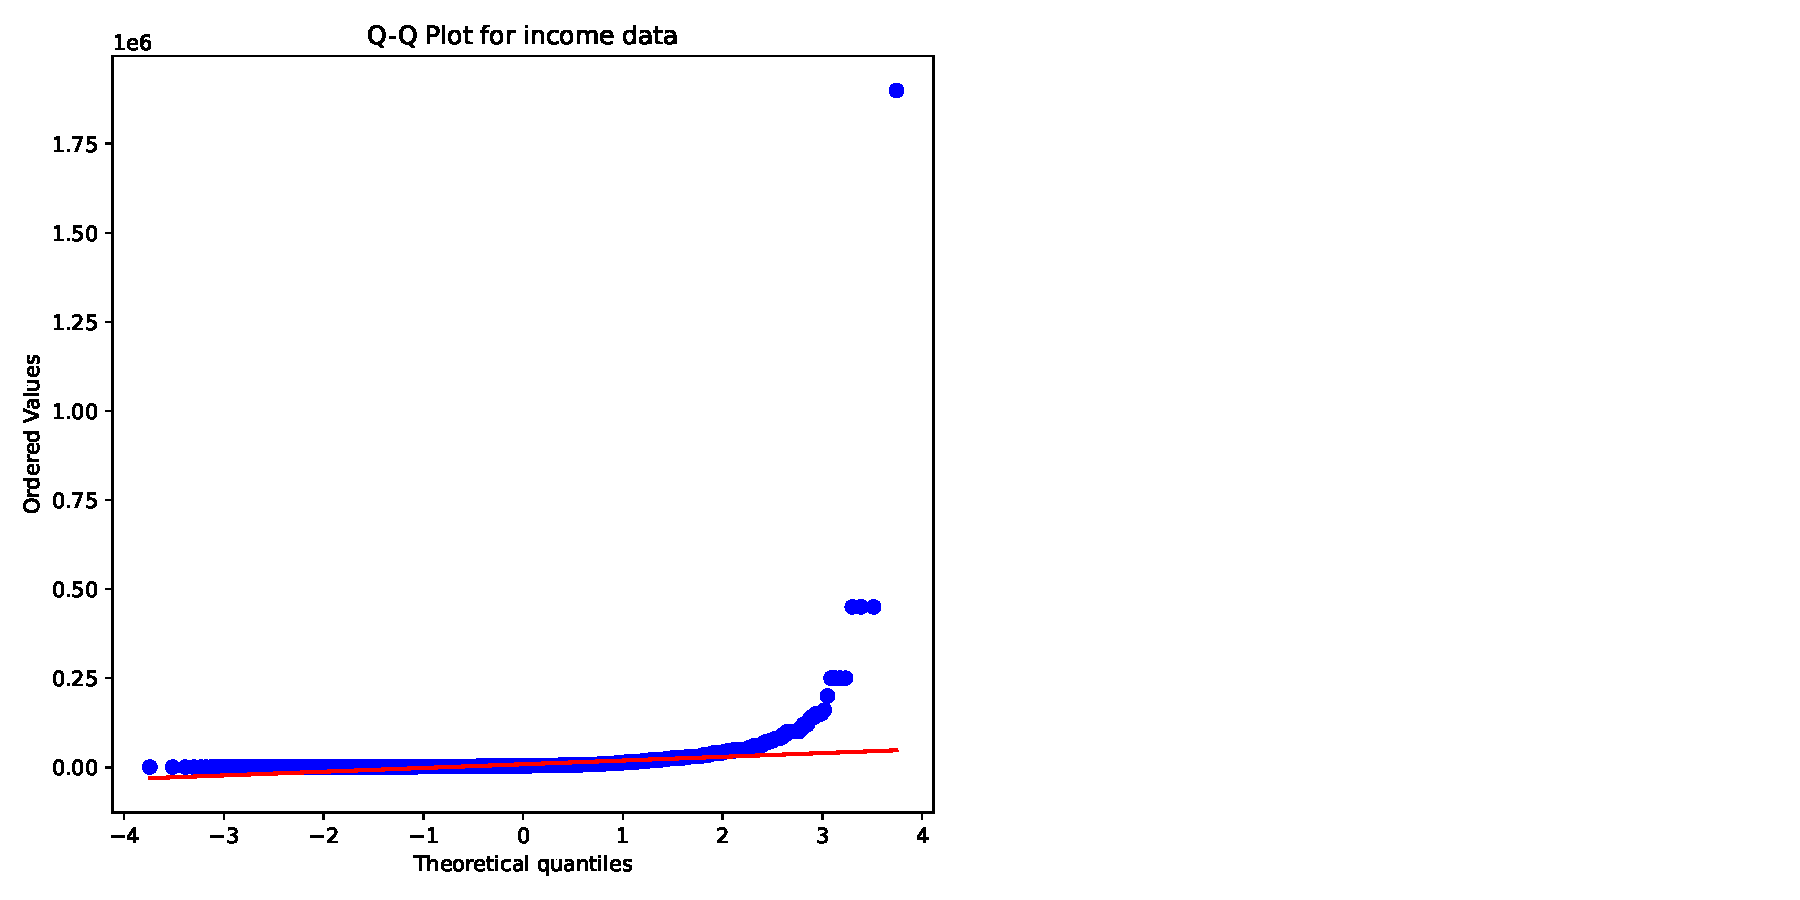
\includegraphics[width=\columnwidth]{images/hyp_2_norm_dist_income data.pdf} % Adjust the path accordingly
%     \caption{Caption for the pdf image.}
%     \label{fig:Independence test for anova test}
% \end{figure}

\begin{table}[H]
    \centering
    \caption{Levene independence test results}
    \label{tab:Levene test results}
    \begin{minipage}{\columnwidth}
        \begin{tabular}{rrrrr}
\toprule
df & sum\_sq & mean\_sq & F & PR(>F) \\
\midrule
5.000 & 271399165518.753 & 54279833103.751 & 79.258 & 0.000 \\
7590.000 & 5198036057205.649 & 684853235.468 & NaN & NaN \\
\bottomrule
\end{tabular}

    \end{minipage}
\end{table}

% \begin{table}[H]
%     \centering
%     \caption{Welch test results}
%     \label{tab:Welch anova test results}
%     \begin{minipage}{\columnwidth}
%         \begin{tabular}{rrrrr}
\toprule
df & sum\_sq & mean\_sq & F & PR(>F) \\
\midrule
5.000 & 271399165518.753 & 54279833103.751 & 79.258 & 0.000 \\
7590.000 & 5198036057205.649 & 684853235.468 & NaN & NaN \\
\bottomrule
\end{tabular}

%     \end{minipage}
% \end{table}

% \begin{table}[H]
%     \centering
%     \caption{Tukey results}
%     \label{tab:Tukey results}
%     \begin{minipage}{\columnwidth}
%         \begin{tabular}{lrrrrrrr}
\toprule
 & group1 & group2 & meandiff & p-adj & lower & upper & reject \\
\midrule
0 & 0.0000 & 1.0000 & 146.5434 & 1.0000 & -8890.4647 & 9183.5515 & False \\
1 & 0.0000 & 2.0000 & 716.2572 & 0.9996 & -5822.8625 & 7255.3770 & False \\
2 & 0.0000 & 3.0000 & 4063.5954 & 0.4301 & -2179.2058 & 10306.3967 & False \\
3 & 0.0000 & 4.0000 & 9090.1826 & 0.0215 & 818.1259 & 17362.2394 & True \\
4 & 0.0000 & 5.0000 & 20251.3632 & 0.0000 & 13676.4532 & 26826.2732 & True \\
5 & 1.0000 & 2.0000 & 569.7139 & 0.9999 & -6410.3448 & 7549.7726 & False \\
6 & 1.0000 & 3.0000 & 3917.0521 & 0.5547 & -2786.2083 & 10620.3125 & False \\
7 & 1.0000 & 4.0000 & 8943.6393 & 0.0369 & 318.7882 & 17568.4903 & True \\
8 & 1.0000 & 5.0000 & 20104.8198 & 0.0000 & 13091.2206 & 27118.4191 & True \\
9 & 2.0000 & 3.0000 & 3347.3382 & 0.0014 & 892.4917 & 5802.1847 & True \\
10 & 2.0000 & 4.0000 & 8373.9254 & 0.0009 & 2417.3637 & 14330.4870 & True \\
11 & 2.0000 & 5.0000 & 19535.1059 & 0.0000 & 16328.3715 & 22741.8404 & True \\
12 & 3.0000 & 4.0000 & 5026.5872 & 0.1114 & -603.0760 & 10656.2504 & False \\
13 & 3.0000 & 5.0000 & 16187.7677 & 0.0000 & 13639.1158 & 18736.4197 & True \\
14 & 4.0000 & 5.0000 & 11161.1806 & 0.0000 & 5165.3502 & 17157.0109 & True \\
\bottomrule
\end{tabular}

%     \end{minipage}
% \end{table}

% The one-way ANOVA indicated a significant effect of education level on salary $F(X, X) = X.XX$, $p < 0.05$. 
% Post-hoc analysis revealed that individuals with higher education levels tend to have higher salaries.

% \subsubsection{Hypothesis 3: Age and Salary}

% A Pearson correlation test revealed a significant positive correlation between age and salary $r = X.XX$, $p < 0.05$, indicating that salary increases with age.

% \subsubsection{Hypothesis 4: Gender and Salary/Education Level}

% The t-test for independent samples indicated a significant effect of gender on salary $t = X.XX$, $p < 0.05$. 
% However, no significant difference was found in education levels between genders.

% \subsubsection{Hypothesis 5: Ethnicity and Salary}

% A multiple regression analysis controlling for education showed a significant effect of ethnicity on salary $\beta = X.XX$, $p < 0.05$, suggesting salary disparities across ethnic groups.

% \subsection{Clustering Results}

% \subsubsection{K-Means Clustering}

% The K-means algorithm identified $X$ distinct clusters based on age and salary. 
% The optimal number of clusters was determined using the silhouette score $S = X.XX$. 
% The clusters revealed patterns of salary progression with age.

% \subsubsection{Hierarchical Clustering}

% Hierarchical clustering produced several distinct groups based on education level, employment status, and age. 
% The dendrogram visualized these relationships clearly.

% \section{Conclusion}

This study systematically examined the impact of various demographic factors—education level, age, gender, and ethnicity—on employment and salary within outcomes using a robust set of statistical methods. The findings contribute valuable insights into socio-economic dynamics within the labor market and highlight the complexities underlying employment trends.

In conclusion, the results of this study underline the multifaceted influences of demographic factors on employment and salary outcomes. The findings not only enrich the existing literature but also inform policymakers, educators, and employers about the critical areas that require intervention to promote equality and improve economic opportunities for all individuals. Future research should aim to further explore these relationships over time and consider additional variables, such as geographic location and industry-specific trends, to provide a more comprehensive understanding of the labor market landscape.

\bibliographystyle{IEEEtran}
\bibliography{refs}

\end{document}